\section{An "Explosive" Transition}
In this paper we are going to take a deeper look into a specific type of percolation called explosive percolation, where the underlying concept is that the onset of percolation is delayed until a certain point where it then occurs at an accelerated rate.
This occurs when the underlying evolution process works in such a way that the largest cluster size $|C|$ is controlled.
We can think of a graph where multiple clusters might evolve separately without merging.
Collectively they take up a large portion of the graph but there isn't a percolating cluster yet due to the lack of connections between the them.
If at some point these clusters do begin to connect then the graph transitions to the percolating state.
For certain evolution processes it has been heavily debated whether or not the phase transition is continuous or not, so the aim of the next section is to summarize what we know to this point regarding the nature of the transition for said processes.

\subsection{How It All Started}
This all started in the year 2000 when Dimitris Achlioptas brought forth an interesting take on adding edges to a random graph.
The basic question was what would happen if instead of randomly adding an edge at each step like in the ER model, one evaluated two edges $\{e_1, e_2\}$ and then added one edge and discarded the other according to some selection criteria.
This process of evaluating $m \ge 2$ edges at each step is referred to as an Achlioptas process.

In 2001 Tom Bohman and Alan Frieze were the first to design and analyze an Achlioptas process in their paper "Avoiding a Giant component" \cite{BF}, which laid out the Bohman-Frieze (BF) model for delaying the appearance of a giant cluster.
At each step edge $e_1$ is added and $e_2$ discarded if $e_1$ connects two clusters of size smaller than $K$, if not $e_2$ is added and $e_1$ discarded.
In their paper they took $K = 2$, thus the algorithm favors connecting isolated nodes rather than connecting clusters containing two or more nodes.
This is known as a "bounded-size" rule which essentially views all clusters of size greater than or equal to $K$ as equivalent.
They were able to show that this method (using $K = 2$) leads to a delayed onset of percolation when compared to the ER model.
This can be seen in Fig. \ref{fig:ER_BF_transition} where the order parameter for the BF model remains smaller than for the ER model, but a little after $t / n = 0.5$ it begins to rise at a faster rate than in the ER model, eventually overtaking the ER model.
It has been hypothesized that all bounded-size rules produce exhibit continuous phase transitions \cite{20070000}.

\begin{figure}[H]
	\centering
	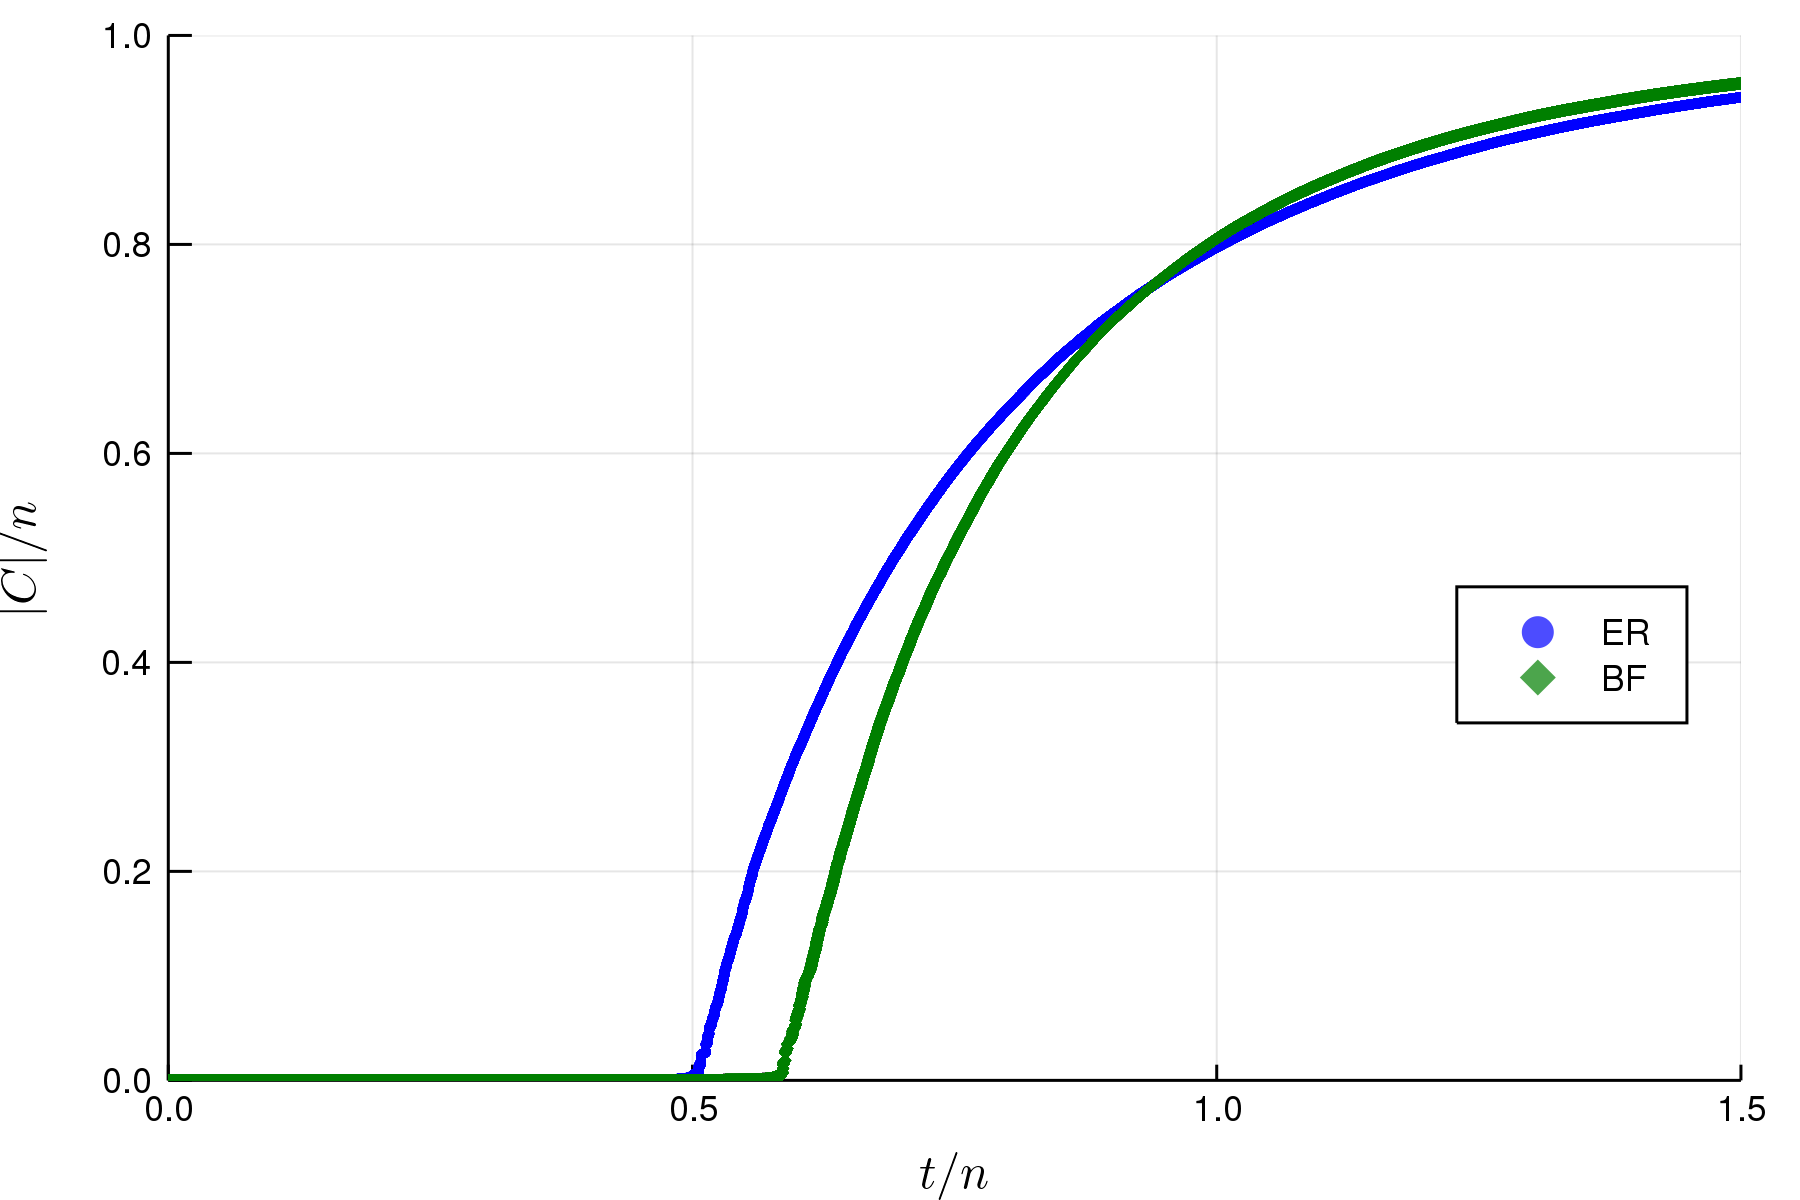
\includegraphics[width=350pt]{images/ER-BF-1e6-order-param.png}
	\caption{Bohman-Frieze Model Order Parameter, $n = 10^6$}
	\label{fig:ER_BF_transition}
\end{figure}

The first mention of explosive percolation appeared in 2009 in the paper "Explosive Percolation in Random Networks" \cite{20090313} by Dimitris Achlioptas, Raissa M. D’Souza, and Joel Spencer, which will henceforth be referred to as Achlioptas et al.
In this paper they laid out a method of choosing edges called the product rule (PR).
At each step in the PR evolution process two edges are selected at random and evaluated based on the product of the cluster sizes that the edges would connect.
More specifically, if edge $e_1$ connects clusters $C_1$ and $C_2$ and edge $e_2$ connects clusters $C_3$ and $C_4$, then $e_1$ is accepted if $|C_1| \cdot |C_2| < |C_3| \cdot |C_4|$, otherwise $e_2$ is accepted.
This process significantly delays the phase transition until all of a sudden it starts to jump up in large amounts.
This can be seen in Fig. \ref{fig:ER_BF_PR_transition} where the order parameter is plotted along side those of the ER and BF models.

\begin{figure}[H]
	\centering
	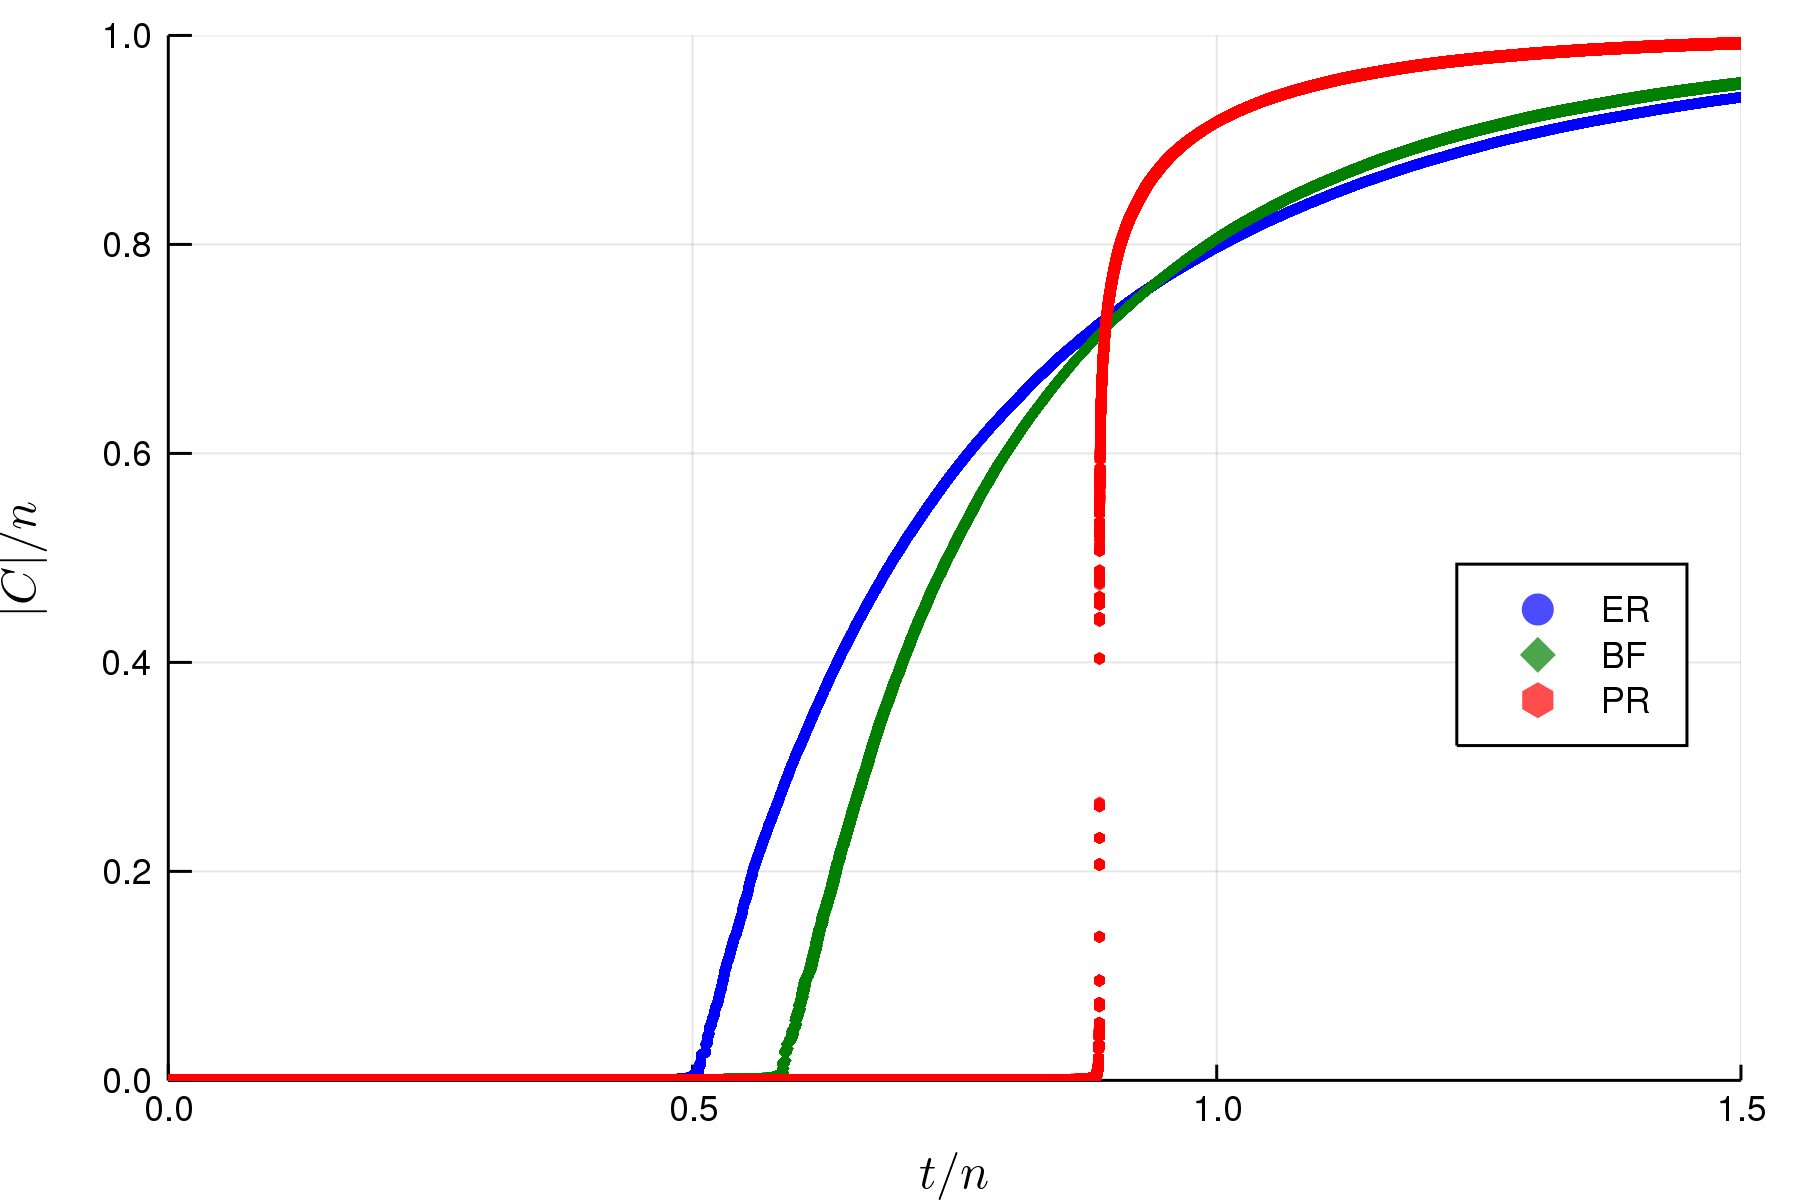
\includegraphics[width=350pt]{images/ER-BF-PR-1e6-order-param.png}
	\caption{Product Rule Model Order Parameter, $n = 10^6$}
	\label{fig:ER_BF_PR_transition}
\end{figure}
